\documentclass[a4paper]{article}

\usepackage[table]{xcolor}%this has to be the first!!!!!!
\usepackage{fullpage} % Package to use full page
%\usepackage{parskip} % Package to tweak paragraph skipping
\usepackage{tikz} % Package for drawing
\usepackage{tikz-3dplot} % Package for drawing
\usetikzlibrary{shapes,arrows,matrix,positioning}
\usepackage{amsmath}
\usepackage{indentfirst}
\usepackage{hyperref}
\usepackage{subcaption}
\usepackage{graphics}
\usepackage{graphicx}
\usepackage{minted}
\usepackage{romannum}
\usepackage{multicol}
\usepackage{mathrsfs}
%color define
\definecolor{codebg}{RGB}{230,255,253}
\definecolor{function}{RGB}{210,0,26}
\definecolor{para}{RGB}{255,137,137}
\definecolor{output}{RGB}{238,224,201}
\setminted[lexer.py:DiffLexer -x]{mathescape=true,breaklines,bgcolor=codebg,linenos}

\tikzset{
  block/.style = {rectangle, draw, fill=output, text width=6cm, text centered, rounded corners, minimum height=4em},
  line/.style = {draw, -latex'},
}

%function newcommand
\newcommand{\func}[1]{\textbf{\textcolor{function}{#1}}}
\newcommand{\para}[1]{\textbf{\emph{\textcolor{para}{#1}}}}
\newcommand{\activetest}{\tikz \fill[black] (3pt,3pt) circle (3pt);}
\newcommand{\prolong}{\tikz \fill[blue] (3pt,3pt) circle (3pt);}
\newcommand{\rest}{\tikz \fill[red] (3pt,3pt) circle (3pt);}

\usepackage{biblatex}
\addbibresource{bibliography.bib}
\title{poisson.h Documentation}
\author{Haochen(Langford) Huang}
\date{\today}

\begin{document}

\maketitle

\section{Introduction and Background}\label{sec:intro}
\textbf{poisson.h} serves as toolbox which provides functions to construct V-cycle iteration sovler for implicit equations. A specific one for solving poisson equation is constructed within the headfile as an example. We shall first introduce the constructing toolbox.\par
Assuming the governing equation can be written as
\begin{equation}
  f( x) = y
\end{equation}
where $y$ is the known variable, $ x$ is the desired variable and $f$ represnts linear operator that satisfies
\begin{equation}\label{equ:cons}
  f( x_a+ x_b) = f( x_a) + f( x_b)
\end{equation}
Now consider the discrete form of operator $\hat{f}$ which takes all desired variable from every cell (suppose the total number of cell is $n$) to express the local known variable $y_i$ then yeilds the implicit equation group
\begin{equation}\label{equ:aim}
  \hat{f}(x_1,x_2,x_3,\cdots,x_n) = y_i \quad i = 1,2,\cdot,n
\end{equation}
which can be solved by nondirective iterative method such as Jacobi method, G-S method\cite{moin2010fundamentals} \emph{etc.} Moreover, constraints \ref{equ:cons} provide another perspective to construct equation group. Use $x_1^e,x_2^e,\cdots,x_n^e$ to denote exact solution of Eq.\ref{equ:aim} and $x_1^k,x_2^k,\cdots,x_n^k$ to represent result of $k$th iteration. Following Eq.\ref{equ:cons} we have
\begin{equation}\label{equ:iter}
  \hat{f}(\delta x_1^k,\delta x_2^k,\cdots, \delta x_n^k) = RES^k
\end{equation}
where $\delta x_i^k = x_i^e - x_i^k$, $RES^k = \hat{f}(x_1^e,x_2^e,\cdots,x_n^e) - \hat{f}(x_1^k,x_2^k,\cdots,x_n^k)$. The criterion of solution then becomes $|RES^k|_{\infty}<\epsilon$ where $\epsilon$ is a setting tolerance.\par
There are many techniques to accelerate the convergence of iteration, and multigrid method\cite{wesseling1995introduction} may be one of the most famous which employs iterations on every layer of the mesh to reduce the residual of corresponding wavenumber. A similiar methodology is applied by quadtree/octree in Basilisk. Take quadtree as anexapmle. Consider tree architecture in Fig.\ref{fig:2dquad}, the actual caculating rules for this problem is shown in \ref{fig:caculation} where $\activetest$ represents leaf cells (the finest cell at this area and is not divided by higher level) and the value it carrying is the the final value shown in the result called active value.
$\prolong$ represents ghost cell served as boundary condition whose value is computed by bilinear interpolation. Finally $\rest$ represents value carried by parent cell. The parent cell, indicated by its name, will be divided into 4(8) children cells in finer layer (level in Basilisk).\cite{van2018towards}\par
A single round of iteration is accomplished by two procedures. First, from highest level to lowest one, assign residual to each cell of current level which form the \emph{R.H.S.} of Eq.\ref{equ:iter}. Second, starting from lowest level to the highest, obtain the result after few iterating (by Jacobi method or GS method) on current level and use it to compute initial value on next level. We shall first dive into second procedure which is more sophisticated.\par
Caculations happens at every level shown in Fig.\ref{fig:caculation}, when it comes to higher level the boundary condition is first set and then undergoes the iteration on cells at same level instead of whole domain. Moreover, the initial value on each level is obtained by prolongation (bilinear mostly) from pervious mesh level.\par
In order to facilitate Eq.\ref{equ:iter} we also need residual, which only exists at leaf cell, of every cell at each level. This procedure is achieve by restrcting\cite{popinet2015quadtree} (averaging mostly) value on 4(8) children cells, which is much simpler compared to bilinear that use in previous description.\par 
\begin{figure}[h]
  \begin{subfigure}[b]{0.5\textwidth}
    \centering 
    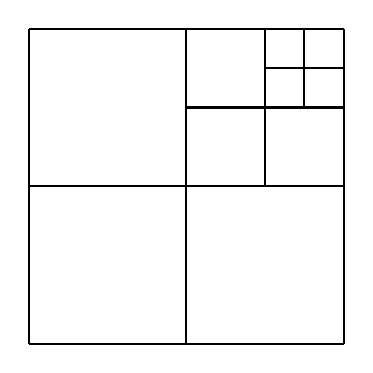
\begin{tikzpicture}
      \draw[thick,step=2cm] (0,0) grid (4,4);
      \draw[thick,step=1cm] (2,2) grid (4,4);
      \draw[thick,step=0.5cm] (3,3) grid (4,4);
    \end{tikzpicture}
    \caption{2D quadtree example.}
    \label{fig:2dquad}
  \end{subfigure}
  \begin{subfigure}[b]{0.5\textwidth}
    \centering 
    \tdplotsetmaincoords{70}{110}
    \begin{tikzpicture}[tdplot_main_coords]
      \foreach \i in {0,2,4}
      {
        \draw[thick] (\i,0,4.5) -- (\i,4,4.5);
        \draw[thick] (0,\i,4.5) -- (4,\i,4.5);
      }
      
      \foreach \i in {1,3}
      {
        \filldraw[black] (1,\i,4.5) circle (2.5pt);
        \filldraw[black] (3,\i,4.5) circle (2.5pt);
      }
      \filldraw[red] (3,3,4.5) circle (2.5pt);

      \foreach \i in {2.5,3.5}
      {
        \draw[gray,dashed] (3,3,4.5)--(\i,2.5,3);
        \draw[gray,dashed] (3,3,4.5)--(\i,3.5,3);

        \filldraw[black] (\i,2.5,3) circle (2pt);
        \filldraw[black] (\i,3.5,3) circle (2pt);

        \filldraw[blue] (\i,1.5,3) circle (2pt);
        \filldraw[blue] (\i,4.5,3) circle (2pt);
        \filldraw[blue] (1.5,\i,3) circle (2pt);
        \filldraw[blue] (4.5,\i,3) circle (2pt);
      }

      \filldraw[red] (3.5,3.5,3) circle (2pt);

      \foreach \i in {2,3,4}
      {
        \draw[thick] (\i,2,3) -- (\i,4,3);
        \draw[thick] (2,\i,3) -- (4,\i,3);
      }

      \foreach \i in {3.25,3.75}
      {
        \draw[gray,dashed] (3.5,3.5,3)--(\i,3.25,1.75);
        \draw[gray,dashed] (3.5,3.5,3)--(\i,3.75,1.75);
        \filldraw[black] (\i,3.25,1.75) circle (1pt);
        \filldraw[black] (\i,3.75,1.75) circle (1pt);

        \filldraw[blue] (\i,2.75,1.75) circle (1pt);
        \filldraw[blue] (\i,4.25,1.75) circle (1pt);
        \filldraw[blue] (2.75,\i,1.75) circle (1pt);
        \filldraw[blue] (4.25,\i,1.75) circle (1pt);
      }

      \foreach \i in {3,3.5,4}
      {
        \draw[thick] (\i,3,1.75) -- (\i,4,1.75);
        \draw[thick] (3,\i,1.75) -- (4,\i,1.75);
      }

      \draw[very thick,-latex] (3,1,3.5)--(3,1,1.0);
    \end{tikzpicture}
    \caption{Caculation for each level. }
    \label{fig:caculation}
  \end{subfigure}
    \caption{Quadtree example. Arrow in (b) indicates caculating sequence.}
    \label{fig:2dexample}
\end{figure}
After introducing the mesh architecture, we shall now step a little further to see the solver structure provided by 'poisson.h' and to perceive the overall workflow. FIG.\ref{fig:workflow} displays whole system as well as its workflow. As can be seen from the sketch, the whole solver consists of four functions, \func{mg\_solve}, \func{mg\_cycle}, \func{relax} and \func{residual}. Their nesting relationg is shown by crresponding position, \emph{e.g.} \func{relax} is inside \func{mg\_cycle} while \func{residual} and \func{mg\_cycle} locate inside \func{mg\_solve} indicates that \func{relax} is called by \func{mg\_cycle} and \func{mg\_cycle} along with \func{residual} are directly called by \func{mg\_solve}. Detailed workflow is also presented, after inputting $ \mathbf{x}^0, \mathbf{y}$ before the residual actually meet the tolerance $\epsilon$, \func{mg\_solve} plays as a manager to make rest functions coordinate, $ \mathbf{x}^k$ is conveyed between \func{mg\_cycle} and \func{residual} to renew. Number behind each step represents the order within the loop. $ \mathbf{x}^k, \mathbf{y}$ is first sent to residual to compute residual $RES^k$ which served as parameter in \func{mg\_cycle}. $ \mathbf{x}^k$ and $n$ are also taken into \func{mg\_cycle}where $n$ controls iteration number on each mesh level. $ \mathbf{x}^{k+1}$ is obtained by first solving Eq.\ref{equ:iter} for $\delta \mathbf{x}^k$ then excute update
\begin{equation}
  \mathbf{x}^{k+1} = \mathbf{x}^k + \delta \mathbf{x}^k
\end{equation}
Loop will break out either residual satisfies tolerance constraint or number of round exceed setting threshold. Readers may notice there is no parameters convyed within \func{mg\_cycle}, this is because relationship between \func{relax} and \func{mg\_cycle} cannot be simply abstracted as 'linear' as depicted in this figure. Structure inside \func{mg\_cycle} is demonstrate in Fig.\ref{fig:mgcycle} as described before residual is assigned to each level then relax is called at each level multiple times updating $\delta \mathbf{x}^k$ in the form (condition varies according to iteration method)
\begin{equation}
  \delta x^k_i = F(\delta x^k_1,\delta x^k_2,\cdots,\delta x^k_{i-1},\delta x^k_{i+1},\cdots,\delta x_n^k, RES^k)
\end{equation}
Back to \func{mg\_solve}, readers may notice from Fig.\ref{fig:workflow} that all the function within, including \func{mg\_solve} itself, are divided into three layer by dashed line and each layer is named by Roman number from top to bottom. Higher the layer, more irreplaceable the function is. Therefore, functions at \Romannum{3} can be changed or altered based on one's purpose. In another word, users can choose their own \func{relax} and \func{residual} based on equation they cope with. The governing equation for \textbf{poisson.h} is
\begin{equation}
  L(a)=\nabla\cdot(\alpha\nabla a) + \lambda a =b
\end{equation}
where $L$ is a linear operator. Based on above discussion such equation can be solved by multigrid solver only if one constructs appropriate \func{relax} and \func{residual} function. Another example is referred to headfile \textbf{viscousity.h} where same solver construction is used for totally different linear equation. 

\begin{figure}[H]
    \centering
    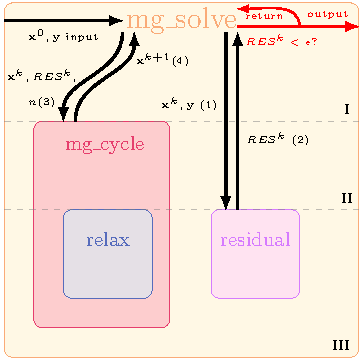
\includegraphics[width=\textwidth]{image/mgsolver.pdf}
    \caption{Architecture of the solver. Nested relationship of functions is indicated by box containing relationship \emph{e.g.} \func{mg\_cycle} contains \func{relax} but not \func{residual} indicates that \func{relax} is called in \func{mg\_cycle} while \func{residual} is called in \func{mg\_solve}.}
    \label{fig:workflow}
\end{figure}

\begin{figure}[H]
    \centering
    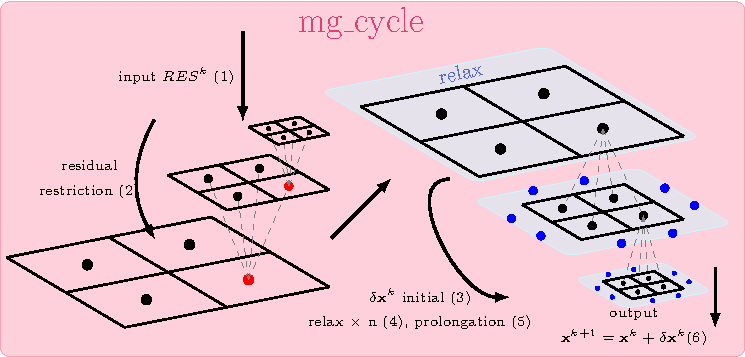
\includegraphics[width=\textwidth]{image/mgcycle.pdf}
    \caption{Combination between \func{mg\_cycle} and \func{relax}. The 'round' of iteration described before is also demonstrated in a detailed way. \func{relax} herein is embed into every level of the mesh and is excuted several times (depends on parameter $n$) on each level to accelerate convergence.}
    \label{fig:mgcycle}
\end{figure}

\section{Functions}\label{sec:func}
\subsection{\func{mg\_cycle}}
\subsubsection{Parameters}
\begin{center}
  \begin{tabular}{|c|c|c|c|c|}
    \hline
    Name & Data type & Status & Option/Default & Representation (before/after)\\[0.5ex]
    \hline\hline
    \rowcolor{output}\para{a} & scalar* & update & complusory & $ \mathbf{x}^{k}/ \mathbf{x}^{k+1}$\\
    \hline
    \para{res} & scalar* & unchange & complusory & $ \delta \mathbf{x}^k$\\
    \hline
    \para{da} & scalar* & unchange & complusory & $\rho^{n+ \frac{1}{2}}$\\
    \hline
    \para{relax} & void* & unchange & complusory &  \func{relax}\\
    \hline
    \para{data} & void* & unchange & complusory &  \func{Poisson} (struct defined below)\\
    \hline
    \para{nrelax} & int & unchange & complusory & $n$ \\
    \hline
    \para{minlevel} & int & unchange & complusory & $minlevel$ \\
    \hline
    \para{maxlevel} & int & unchange & complusory & $maxlevel$ \\
    \hline
  \end{tabular}
\end{center}

\subsubsection{Worth Mentioning Details}
\printbibliography
\end{document}
